\documentclass[12pt,a4paper]{scrartcl}
\usepackage{scrlayer-scrpage}
\pagestyle{scrheadings}
\ohead{Baumann Martin, 01527563}
\ihead{MLA Homework 2 Report}

\usepackage{lmodern}
\usepackage{float}


\usepackage{graphicx}
\usepackage{subfig}
\usepackage[T1]{fontenc}

\usepackage{epstopdf}
\usepackage{amsmath}
\usepackage{amssymb}
\usepackage{siunitx}
\sisetup{exponent-product = \cdot, output-product = \cdot}
\usepackage{prettyref}
\newrefformat{fig}{Figure \ref{#1}}
\newrefformat{tab}{Table \ref{#1}}
\newrefformat{eq}{equation (\ref{#1})}

\usepackage{multirow}
\newcommand{\matr}[1]{\mathbf{#1}}

\usepackage{physics}
\usepackage{tikz}

\begin{document}
	
	\section*{Problem 2.1}
	\subsection*{Softplus function}
	The function
	\begin{equation}
		\max(0, t)
	\end{equation}
	is approximated by the so called softplus function
	\begin{equation}
		\log(1+e^t).
		\label{eq:softplus}
	\end{equation}

	\begin{figure}[H]
		\centering	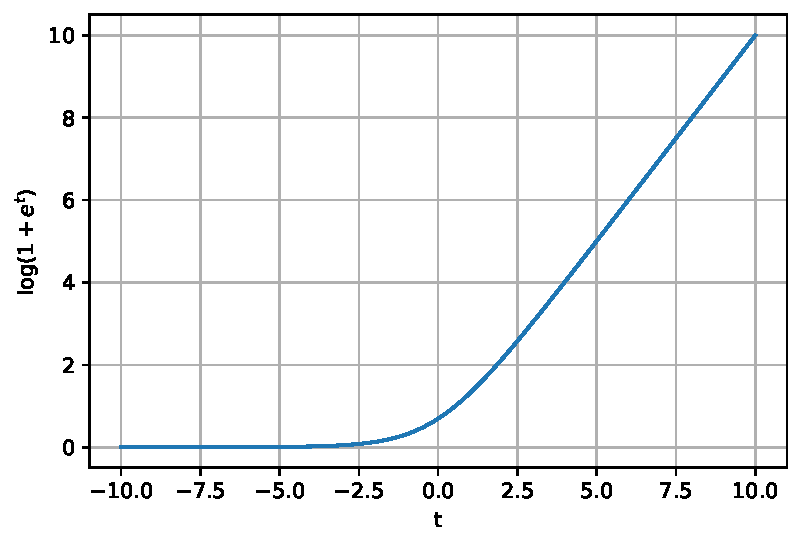
\includegraphics[width=0.85\linewidth]{figs/ex2_1_softplus.pdf}
		\caption{Softplus function \prettyref{eq:softplus}}
		\label{fig:ex2_1_softplus}
	\end{figure}
	
	For $t>0$ it approaches $t$ and for $t<0$ it approaches 0. Therefore the function saturates for t < 0.
	As $t=-y_{(i)} \tilde{y}_{(i)}$ in the loss function, it saturates for $y_{\left(i\right)} \tilde{y}_{(i)} > 0$. Therefore, whenever the predicted soft label and the true label have the same sign  $\mathrm{sign}({y_{(i)}}) = \mathrm{sign}(\tilde{y}_{(i)})$, the loss function saturates and only has little effect on the overall loss.

	\subsection*{Analytic gradient}
	The loss function is given by
	\begin{equation}
		J(\matr{w}, b) = \frac{1}{N} \sum_{i=1}^{N} \log \left(1+e^{-y_{(i)}\left( \matr{x}_{(i)}^T \matr{w} + b\right) }\right).
	\end{equation}

	The gradient with respect to the weights is
	\begin{align}
		\nabla_\matr{w} 	J(\matr{w}, b) =&  \frac{1}{N} \sum_{i=1}^{N} \frac{1}{1+e^{-y_{(i)}\left( \matr{x}_{(i)}^T \matr{w} + b\right) }} \nabla_\matr{w} e^{-y_{(i)}\left( \matr{x}_{(i)}^T \matr{w} + b\right) } = \\
		&\frac{1}{N} \sum_{i=1}^{N} \frac{e^{-y_{(i)}\left( \matr{x}_{(i)}^T \matr{w} + b\right) }}{1+e^{-y_{(i)}\left( \matr{x}_{(i)}^T \matr{w} + b\right) }} \left(-y_{(i)} \matr{x}_{(i)}\right).
	\end{align}

	The gradient with respect to the bias term can be computed completely analogous, except that in the inner derivate there is no $\matr{x}_{(i)}$ term
		\begin{align}
		\nabla_b 	J(\matr{w}, b) =\frac{1}{N} \sum_{i=1}^{N} \frac{e^{-y_{(i)}\left( \matr{x}_{(i)}^T \matr{w} + b\right) }}{1+e^{-y_{(i)}\left( \matr{x}_{(i)}^T \matr{w} + b\right) }} \left(-y_{(i)}\right).
	\end{align}

	\subsection*{Gradient descent}
	
	A gradient descent algorithm has been implemented. After $K=600$ iterations the parameters $\hat{\matr{w}}^{\left(K\right)} = [-2.13, 0.04]^T$ and $\hat{b}^{\left(K\right)}=1.25$ have been found.
	The classifier achieves an accuracy of \SI{100}{\percent}, i.e. it correctly classifies all samples from the training set.
	In \prettyref{fig:ex2_1_grad_desc} the loss and parameters are shown during the gradient descent iteration. The loss decreases monotonically and almost approaches zero.
	The parameters do not reach a steady state during $600$ iterations. They still change slowly towards the end.
	
	\begin{figure}[H]
		\centering	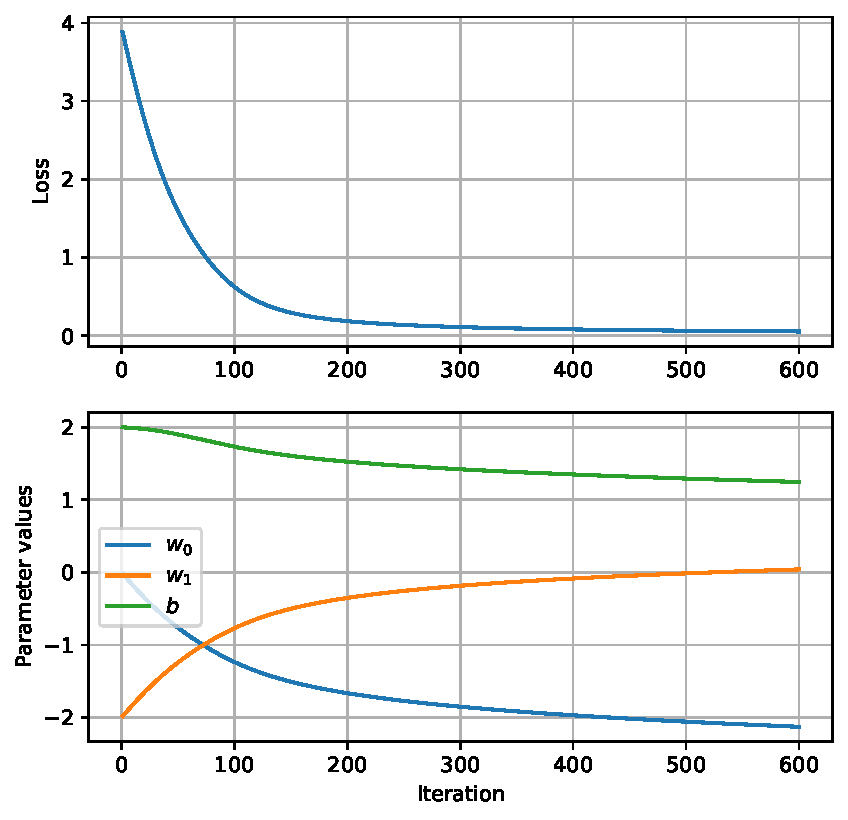
\includegraphics[width=0.85\linewidth]{figs/ex2_1_grad_desc.pdf}
		\caption{Loss and parameters during gradient descent}
		\label{fig:ex2_1_grad_desc}
	\end{figure}
	
	\subsection*{Decision surface}
	
	The decision surface is shown in \prettyref{fig:ex2_1_boundary}. The data can be separated by the classifier and from this plot it too can be seen that the classifier achieves an accuracy of \SI{100}{\percent }.
	The decision surface is very close to the red data. 
	As was shown in \prettyref{fig:ex2_1_softplus}, the loss function approaches zero for $t < 0$ and the gradient becomes very small. 
	Therefore, as the classifier already perfectly classifies all the samples in the test set, the gradient is very small. That is why in \prettyref{fig:ex2_1_grad_desc} the parameters change slowly towards the end.	
	
	A decision surface which maximizes the margin might be preferable in some cases due too higher robustness. This can be done by penalizing $||\matr{w}||$ in the loss function and therefore maximizing the margin around the decision surface (Support Vector Classification).
	
	\begin{figure}[H]
		\centering	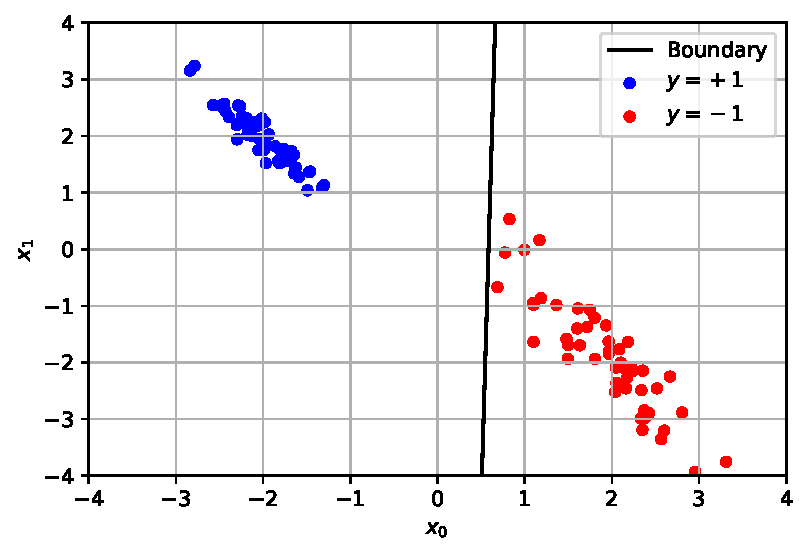
\includegraphics[width=0.85\linewidth]{figs/ex2_1_boundary.pdf}
		\caption{Decision surface and data points of the training set}
		\label{fig:ex2_1_boundary}
	\end{figure}
	
	\subsection*{Loss comparison}
	
	For the two samples
	$s_1=\{[-100,0]^T, 1\}; s_2=\{[-1, 0]^T, -1\}$ the loss is shown in \prettyref{tab:ex2_1_losses}. 
	
	The sample $s_1$ is correctly classified, the loss of that samples is zero, this corresponds to the $t<0$ region of the softplus function. In this region the function is approximately zero.
	The sample $s_2$ is wrongly classified, the loss is $3.41$, this corresponds to the $t>0$ region of the softplus function. In this region the loss is approximately proportional to the distance of the sample from the decision surface.
	
	Compared to the least squares classifier, this cost function does not penalize correctly classified samples and wrongly classified samples are penalized proportionally to the distance form the decision surface. Therefore, this loss function is superior.
	
	\begin{table}[H]
		\centering
		\begin{tabular}{|l|l|}
			\hline
			& Loss \\ \hline
			$s_1$ & 0.0  \\ \hline
			$s_2$ & 3.41 \\ \hline
		\end{tabular}
		\caption{Loss of the two samples}
		\label{tab:ex2_1_losses}
	\end{table}
	
	\section*{Problem 2.2}
	
	\subsection*{SVC blobs dataset}
	
	In \prettyref{fig:ex2_2_blobs} the dataset is shown with the decision surface. The decision surface separates the two labels and is exactly in between the two regions. The inclusion of the $||\matr{w}||$ term in the loss leads to a decision boundary that is maximizing the margin.
	The two translated version of the hyperplane pass through some of the datapoints, those are the so called support vectors.	The margin is the distance between the two translated lines and can be calculated by $\frac{2}{||\matr{w}||}$. In this case the margin is $1.47$.
		
	\begin{figure}[H]
		\centering	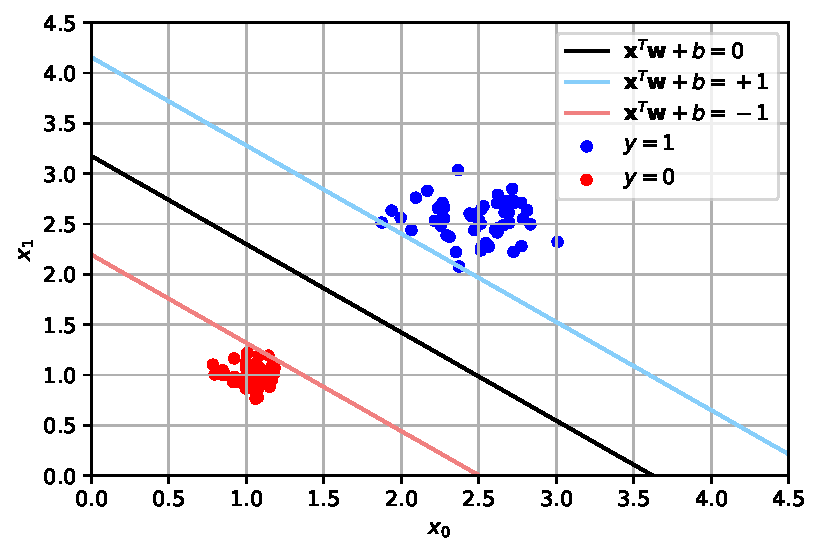
\includegraphics[width=0.85\linewidth]{figs/ex2_2_blob_boundary.pdf}
		\caption{Blobs dataset with decision surface of SVC. The two symmetric translations are shown too}
		\label{fig:ex2_2_blobs}
	\end{figure}

	The weights and bias are shown in \prettyref{tab:ex2_2_blobs_weights}.
	\begin{table}[H]
		\centering
		\begin{tabular}{|l|l|}
			\hline
			$w_0$ & 0.89  \\ \hline
			$w_1$ & 1.02 \\ \hline
			$b$ & -3.24 \\ \hline
		\end{tabular}
		\caption{Weights and bias of the linear SVC}
		\label{tab:ex2_2_blobs_weights}
	\end{table}
	
	\subsection*{Linear SVC circles dataset}
	
	The circles dataset with the decision surface of the linear SVC is shown in \prettyref{fig:ex2_2_circles_lin}. The data is not linearly separable, therefore a linear SVC makes no sense and the produced result is poor.
	
	\begin{figure}[H]
		\centering	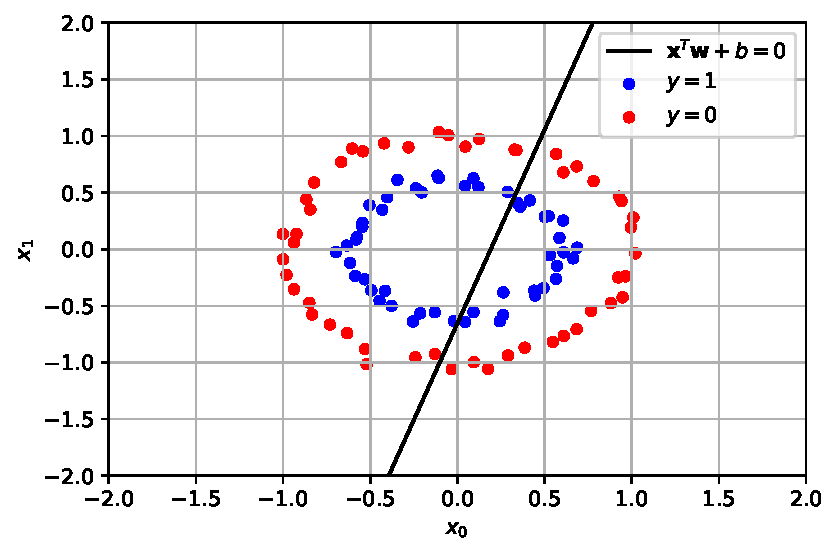
\includegraphics[width=0.85\linewidth]{figs/ex2_2_circ_boundary.pdf}
		\caption{Circles dataset with decision surface of linear SVC. The data is not linearly separable, therefore a linear SVC makes no sense}
		\label{fig:ex2_2_circles_lin}
	\end{figure}
	
	\subsection*{SVC circles dataset with transformation}
	As can be seen in the previous Figure, the separating feature is the radius.
	Therefore introducing the transformation
	\begin{equation}
		\phi(x) = [x_0, x_1, x_2]^T = [x_0, x_1, x_0^2+x_1^2]^T
	\end{equation}
	
	makes the data linearly separable.
	In \prettyref{fig:ex2_2_circles_transformed} the transformed data is shown in the transformed space $x_0, x_2$, with $x_1=0$. The decision surface as well as the two translations are also shown. With this transformation the data is linearly separable, and a linear SVC can be used.
	The data points are projected to the plane with $x_1=0$ that is why some points appear to be inside the margin.	
	
	\begin{figure}[H]
		\centering	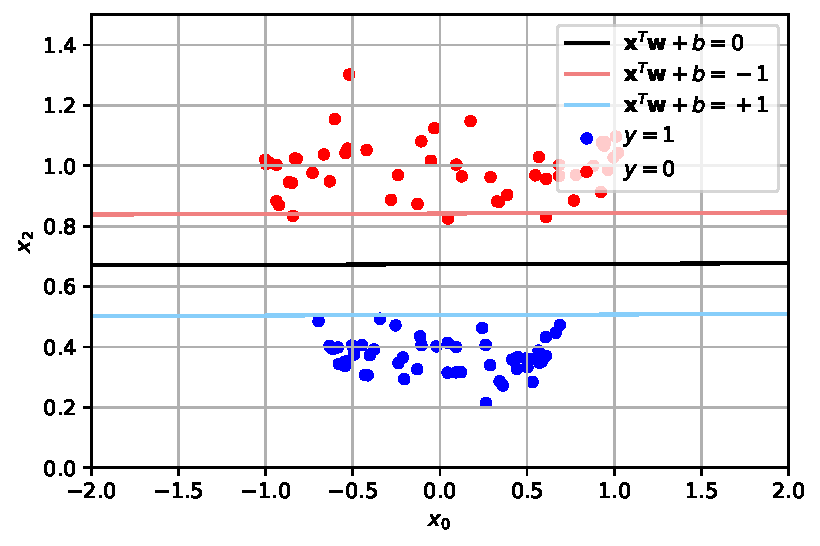
\includegraphics[width=0.85\linewidth]{figs/ex2_2_circ_ext.pdf}
		\caption{Circles dataset in the transformed space. In this space the data is linearly separable.}
		\label{fig:ex2_2_circles_transformed}
	\end{figure}
	
	\subsection*{SVC with polynomial kernel on circles dataset}
	A polynomial kernel with degree two was used to obtain the heatmap in \prettyref{fig:ex2_2_heatmap}.
	The predicted output is $1$ inside a circle and $0$ outside. Like the transformation used in the previous section, the polynomial kernel is also able to capture the nonlinear shape of the decision surface.
	
	\begin{figure}[H]
		\centering	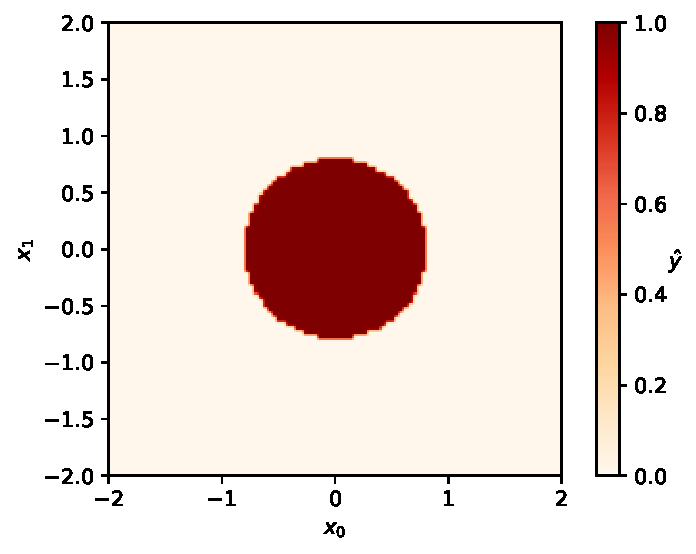
\includegraphics[width=0.8\linewidth]{figs/ex2_2_circ_heatmap.pdf}
		\caption{Heatmap of predicted labels for the SVC with polynomial kernel of degree 2}
		\label{fig:ex2_2_heatmap}
	\end{figure}
	
	\subsection*{Kernel function}
	The nonlinear transformation is implicitly defined via ther kernel function
	\begin{equation}
		k(\matr{x}_{(i)}, \matr{x}_{(j)}) = \langle \phi \left(\matr{x}_{(i)}\right)\,\phi \left(\matr{x}_{(j)}\right)\rangle.
	\end{equation}
	
	The polynomial kernel of degree 2 is defined as
	\begin{align}
		k(\matr{x}_{(i)}, \matr{x}_{(j)}) = \left(\matr{x}_{(i)}^T \matr{x}_{(j)} +1 \right)^2.
	\end{align}
	For $\matr{x} = \left[x_0, x_1\right]^T$ the transformation an be found by expanding
	\begin{align}
		&\left(\matr{x}_{(i)}^T \matr{x}_{(j)} +1 \right)^2 = \left(\matr{x}_{(i)}^T \matr{x}_{(j)}\right)^2+2\matr{x}_{(i)}^T \matr{x}_{(j)} + 1 = \\& \left(x_{0,(i)} x_{0,(j)} + x_{1,(i)} x_{1,(j)}\right)^2 + 2x_{0,(i)} x_{0,(j)} + 2x_{1,(i)} x_{1,(j)} + 1 = \\
		&\left(x_{0,(i)} x_{0,(j)}\right)^2+2x_{0,(i)} x_{0,(j)}x_{1,(i)} x_{1,(j)} + \left(x_{1,(i)} x_{1,(j)}\right)^2+2x_{0,(i)} x_{0,(j)} + 2x_{1,(i)} x_{1,(j)} + 1.
	\end{align}
	
	Therefore the transformation defined by the kernel is
	\begin{equation}
		\phi(\matr{x}) = \left[x_0^2, \sqrt{2}x_0 x_1, x_1^2, \sqrt{2} x_0, \sqrt{2} x_1, 1 \right]^T.
	\end{equation}
	
	The 2 dimensional vector is transformed to a 6-d vector ($d_2=6$).
	
	\section*{Problem 1.3}
	
	\subsection*{Dataset histogram}
	
	A histogram of the train and test set is shown in \prettyref{fig:ex2_3_hist}. For both dataset there are far more samples with $y=0$ compared to $y=1$. For both only \SI{1}{\percent} of the samples have the label $1$.  The dataset is imbalanced.
	
	\begin{figure}[H]
		\centering	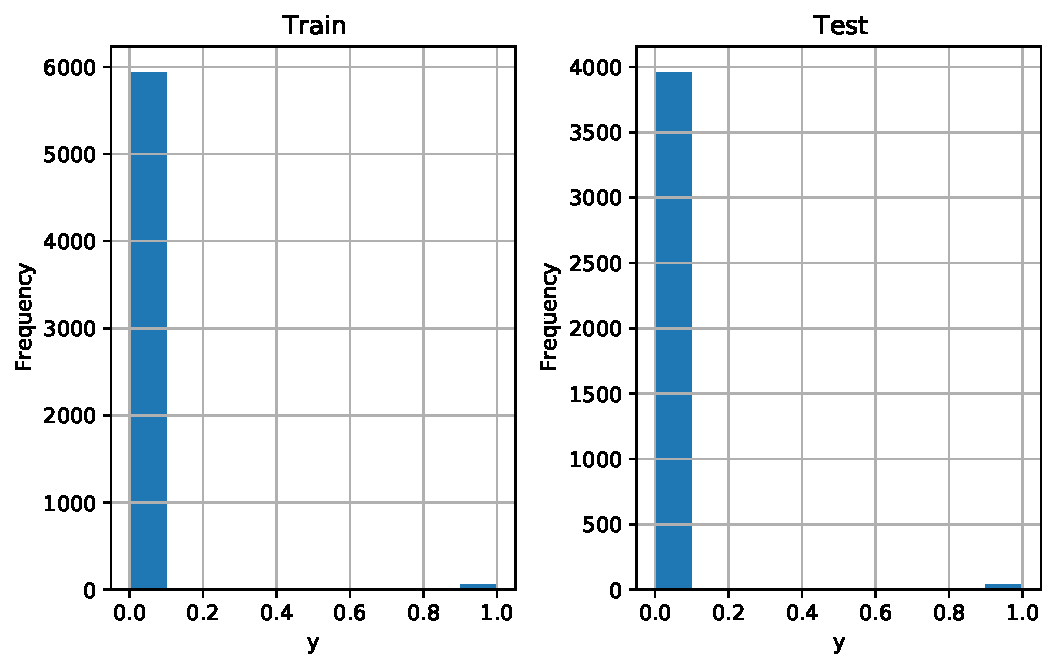
\includegraphics[width=0.85\linewidth]{figs/ex2_3_hist.pdf}
		\caption{Histogram of train and test dataset}
		\label{fig:ex2_3_hist}
	\end{figure}
	
	\subsection*{Original dataset}
	A SVC with RBF kernel was used as a classifier and was trained on the original dataset.
	In \prettyref{tab:ex2_3_conf_m1} the confusion matrix is shown for this classifier evaluated on the test set. In \prettyref{tab:ex2_3_perf1} some performance metrics are noted. 
	
	While just looking at the accuracy the performance of the classifier seems to be good with \SI{99}{\percent}. This is just due to the fact that only \SI{1}{\percent} of the samples have the label $y=1$.  In fact by looking at the confusion matrix it can be seen that the classifier predicts $\hat{y}=0$ for every sample. The classifier has just learned that $y=1$ is much more likely independent of the features.
	The other performance metrics cannot be evaluated.
	
	\begin{table}[H]
		\centering
		\begin{tabular}{c|c|c|}
			& $\hat{y}=0$ & $\hat{y}=1$ \\ \hline
			$y=0$ & 3960      & 0         \\ \hline
			$y=1$ & 40        & 0         \\ \hline
		\end{tabular}
		\caption{Confusion Matrix for SVC trained on original dataset}
		\label{tab:ex2_3_conf_m1}
	\end{table}
	
	\begin{table}[H]
		\centering
		\begin{tabular}{|c|c|}
			\hline
			Accuracy  & 0.99 \\ \hline
			Precision & NaN \\ \hline
			Recall    & 0.00 \\ \hline
			F1-Score  & NaN \\ \hline
		\end{tabular}
		\caption{Performance-Metrics for SVC trained on original dataset}
		\label{tab:ex2_3_perf1}
	\end{table}
	
	\subsection*{Undersampling}
	Undersampling was implemented on the train dataset to train the classifier. The same SVC as in the previous task has been used. Again in \prettyref{tab:ex2_3_conf_m2} and \prettyref{tab:ex2_3_perf2} the results are reported.
	
	The accuracy actually got a bit worse, but the other performance metrics improved.
	Precision is the fraction of true positives divided by total predicted positive. This value is low, meaning that the classifier predicts $1$  too often for data that is actually negative $y=0$.
	Recall is the fraction of true positives divided by total positive. This value is relatively high with $0.73$ meaning that of the samples that are actually $1$ most of the are correctly classified to be $1$.
	The F1-Score is the geometric mean of both measures.
		
	\begin{table}[H]
		\centering
		\begin{tabular}{c|c|c|}
			& $\hat{y}=0$ & $\hat{y}=1$ \\ \hline
			$y=0$ & 3491      & 469         \\ \hline
			$y=1$ & 11        & 29         \\ \hline
		\end{tabular}
		\caption{Confusion Matrix for SVC trained with undersampling}
		\label{tab:ex2_3_conf_m2}
	\end{table}

	\begin{table}[H]
		\centering
		\begin{tabular}{|c|c|}
			\hline
			Accuracy  & 0.88 \\ \hline
			Precision & 0.06 \\ \hline
			Recall    & 0.73 \\ \hline
			F1-Score  & 0.11 \\ \hline
		\end{tabular}
		\caption{Performance-Metrics for SVC trained with with undersampling}
		\label{tab:ex2_3_perf2}
	\end{table}

	\subsection*{Oversampling}
	The results for oversampling are reported in \prettyref{tab:ex2_3_conf_m3} and \prettyref{tab:ex2_3_perf3}.
	
	With this method both false positives and false negatives decreased, thus increasing precision and recall compared to undersampling.
	
	Subsequently also the F1-Score is higher, meaning that for this dataset the highest F1-Score can be achieved with oversampling.
	
	
	\begin{table}[H]
		\centering
		\begin{tabular}{c|c|c|}
			& $\hat{y}=0$ & $\hat{y}=1$ \\ \hline
			$y=0$ & 3759      & 201         \\ \hline
			$y=1$ & 9        & 31         \\ \hline
		\end{tabular}
		\caption{Confusion Matrix for SVC trained with oversampling}
		\label{tab:ex2_3_conf_m3}
	\end{table}

	\begin{table}[H]
		\centering
		\begin{tabular}{|c|c|}
			\hline
			Accuracy  & 0.95 \\ \hline
			Precision & 0.13 \\ \hline
			Recall    & 0.78 \\ \hline
			F1-Score  & 0.23 \\ \hline
		\end{tabular}
		\caption{Performance-Metrics for SVC trained with with oversampling}
		\label{tab:ex2_3_perf3}
	\end{table}

	
	

\end{document}